\PassOptionsToPackage{force}{filehook}

\documentclass{beamer}
\usepackage[utf8]{inputenc}
\usepackage{decimal}
%\usepackage[spanish]{babel}
%\spanishdecimal{.}
%\decimalpoint
\usepackage{amsmath}
\usepackage{amssymb}% http://ctan.org/pkg/amssymb
\usepackage{amsfonts}
\usepackage{pifont}% http://ctan.org/pkg/pifont
%https://tex.stackexchange.com/questions/42619/x-mark-to-match-checkmark
\newcommand{\cmark}{\ding{51}}
\newcommand{\xmark}{\ding{55}}
%\usepackage{amsfonts}
\usepackage{graphicx} 
\usepackage{subcaption}
\usepackage{hyperref}
\usepackage{cancel}
\usepackage{wrapfig}
\usepackage{enumitem}
\usepackage{comment}
\hypersetup{
	colorlinks=true,
	linkcolor=blue,
	filecolor=magenta,      
	urlcolor=cyan,
}
\newtheorem*{proposicion}{Proposici\'on}
\newtheorem*{teorema}{Teorema}
\renewcommand*{\proofname}{Demostraci\'on}
\newtheorem*{ejercicio}{Ejercicio}
\usepackage{pgf,tikz}
\usetikzlibrary{positioning}
\usetikzlibrary{arrows,patterns}
\usetikzlibrary{arrows.meta}
\usepackage[spanish, activeacute]{babel} %Definir idioma español
\decimalpoint
\usepackage[utf8]{inputenc} %Codificacion utf-8
\usepackage{multirow}

%   Esconder las soluciones
\newif\ifhideproofs
\hideproofstrue %uncomment to hide proofs

\ifhideproofs
\usepackage{environ}
\NewEnviron{hide}{}
\let\solucion\hide
\let\endsolucion\endhide
\fi

\usepackage{color}
\usepackage{mathpazo}
\usepackage{hyperref}
\usepackage{multimedia}
\usepackage{graphicx}
\usepackage{textcomp}
\usepackage[spanish, activeacute]{babel} 
\usepackage{graphicx} 
\usepackage{booktabs}
\usepackage{cite}
\usepackage{hyperref}
\usepackage{multicol}
\usepackage{multirow,array}

\usepackage{mathrsfs}
%\usepackage{amssymb}

\usepackage{tabularx}
    \newcolumntype{L}{>{\raggedright\arraybackslash}X}
        %\newcolumntype{b}{>{\hsize=1.5\hsize}X}
    %\newcolumntype{s}{>{\hsize=.9\hsize}X}

\usepackage{amsthm}
\newtheorem{thm}{Teorema}
\newtheorem{lem}[thm]{Lema}
\newtheorem{axiom}[thm]{Axioma}
\newtheorem{prop}[thm]{Proposici\'on}
\newtheorem{coro}[thm]{Corolario}
\theoremstyle{definition}
\newtheorem{defn}{Definici\'on}
\DeclareGraphicsExtensions{.pdf,.jpeg,.png,.eps}
\usetheme{CambridgeUS}
\setbeamertemplate{navigation symbols}{}

%Paréntisis y otros
\newcommand{\cmc}{\overset{m.c.}{\rightarrow}}
\newcommand{\p}[1]{\left(#1\right)}
\newcommand{\cor}[1]{\left[#1\right]}
\newcommand{\lla}[1]{\left\{#1\right\}}
\newcommand{\eps}{\varepsilon}
\newcommand{\lol}{\mathcal{L}}
\newcommand{\RR}{\mathbb{R}}
\newcommand{\QQ}{\mathbb{Q}}
\newcommand{\NN}{\mathbb{N}}
\newcommand{\paren}[1]{\left(#1\right)}
\newcommand{\corc}[1]{\left[#1\right]}
\newcommand{\llav}[1]{\left\lbrace#1\right\rbrace}
\newcommand{\partt}[1]{\left(\text{#1}\right)}
\newcommand{\corctt}[1]{\left[\text{#1}\right]}
\newcommand{\llavtt}[1]{\left\lbrace\text{#1}\right\rbrace}
\makeatletter
\def\munderbar#1{\underline{\sbox\tw@{$#1$}\dp\tw@\z@\box\tw@}}
\makeatother

%\usepackage[scr=rsfs,cal=boondox]{mathalfa}
\usepackage[scr=esstix,cal=boondox]{mathalfa}

% \usepackage{mdframed}
% \newmdtheoremenv{solucion}{Soluci\'on}

% Enmarcar las soluciones
% \newenvironment{solu}
% {%
% \begin{framed}
%   \begin{solucion}
%   }%
%     {%     
%   \end{solucion}
% \end{framed}
% }

%   Esconder las soluciones
\newif\ifhideproofs
%\hideproofstrue %uncomment to hide proofs

\ifhideproofs
\usepackage{environ}
\NewEnviron{hide}{}
\let\solucion\hide
\let\endsolucion\endhide
\fi



%Graficos y cosas
\usepackage{amssymb}
\usepackage{tikz}
\usepackage{pgfplots}
\usepackage{mathtools}
\usepackage{xcolor}
%\pgfplotsset{compat=1.9}
\usepgfplotslibrary{fillbetween,decorations.softclip}
\pgfplotsset{compat = newest}
\usepackage{pst-func}
\usepackage{pstricks}
\usepackage{pst-plot}

% Comando para usar multiples footnotes en un align environment

\makeatletter
\newcommand{\AlignFootnote}[1]{%
    \ifmeasuring@
    \else
        \footnote{#1}%
    \fi
}
\makeatother

%https://tex.stackexchange.com/questions/82782/footnote-in-align-environment


\DeclareGraphicsExtensions{.pdf,.jpeg,.png,.eps}
\usepackage{tikz}
%\usepackage{tikz-cd}
\usetikzlibrary{decorations}
%\usetikzlibrary{snakes}
\usetikzlibrary{cd}

\useoutertheme{split}
\useinnertheme{rounded}


%\beamertemplatenavigationsymbolsempty  %removes navigation bar
\definecolor{rosee}{rgb}{0.7,0.05,0.25}
\definecolor{pacificorange}{cmyk}{0,.6,1,0} %approved Pacific colors 2010
\definecolor{pacificgray}{cmyk}{0,.15,.35,.60}
\definecolor{pacificlgray}{cmyk}{0,0,.2,.4}
\definecolor{pacificcream}{cmyk}{.05,.05,.15,0}
\definecolor{deepyellow}{cmyk}{0,.17,.80,0}
\definecolor{lightblue}{cmyk}{.49,.01,0,0}
\definecolor{lightbrown}{cmyk}{.09,.15,.34,0}
\definecolor{deepviolet}{cmyk}{.79,1,0,.15}
\definecolor{deeporange}{cmyk}{0,.59,1,18}
\definecolor{dustyred}{cmyk}{0,.7,.45,.4}
\definecolor{grassgreen}{RGB}{92,135,39}
\definecolor{pacificblue}{RGB}{59,110,143}
\definecolor{pacificgreen}{cmyk}{.15,0,.45,.30}
\definecolor{deepblue}{cmyk}{1,.57,0,2}
\definecolor{turquoise}{cmyk}{.43,0,.24,0}
\definecolor{gren}{rgb}{0.2,0.8,0.5}
\definecolor{orang}{rgb}{1,0.64,0}
\definecolor{amethyst}{rgb}{0.6, 0.4, 0.8}
\definecolor{dodgerblue}{rgb}{0.12, 0.56, 1.0}
\definecolor{fandango}{rgb}{0.71, 0.2, 0.54}
\definecolor{forestgreen(traditional)}{rgb}{0.0, 0.27, 0.13}
\definecolor{iris}{rgb}{0.35, 0.31, 0.81}
\definecolor{jazzberryjam}{rgb}{0.65, 0.04, 0.37}
\definecolor{mediumjunglegreen}{rgb}{0.11, 0.21, 0.18}
\definecolor{mediumpersianblue}{rgb}{0.0, 0.4, 0.65}
\definecolor{midnightgreen}{rgb}{0.0, 0.29, 0.33}
\definecolor{orangee}{rgb}{1.0, 0.5, 0.0}

% There are many different themes available for Beamer. A comprehensive
% list with examples is given here:
% http://deic.uab.es/~iblanes/beamer_gallery/index_by_theme.html
% You can uncomment the themes below if you would like to use a different
% one:
%\usetheme{AnnArbor} %boca
%\usetheme{Antibes} %azul y gris
%\usetheme{Bergen} %barra who where
%\usetheme{Berkeley} %bordes
%usetheme{Berlin} %blanco y azul
%\usetheme{Boadilla}
%\usetheme{boxes}
\usetheme{CambridgeUS}
%\usetheme{Copenhagen}
%\usetheme{Darmstadt}
%\usetheme{default}
%\usetheme{Frankfurt}
%\usetheme{Goettingen}
%\usetheme{Hannover}
%\usetheme{Luebeck}
%\usetheme{Malmoe}
%\usetheme{Marburg}
%\usetheme{Montpellier}
%\usetheme{PaloAlto}
%\usetheme{Pittsburgh}
%\usetheme{Rochester}
%\usetheme{Singapore}
%\usetheme{Szeged}
%\usetheme{Warsaw}

%\usecolortheme{beaver}
%\usecolortheme{whale}
%\usecolortheme{orchid}
%\usecolortheme{wolverine}
%\usecolortheme[named=pacificblue]{structure} %replaces the blue of Copenhagen with Pacific orange

\definecolor{myNewColorA}{rgb}{0,0,100}
\definecolor{myNewColorB}{rgb}{0,100,100}
\definecolor{myNewColorC}{rgb}{0,200,100}
\definecolor{myNewColorD}{rgb}{0,100,200}

%\setbeamercolor*{palette primary}{bg=myNewColorA, fg = black}
%\setbeamercolor*{palette secondary}{bg=myNewColorB, fg = black}
%\setbeamercolor*{palette tertiary}{bg=myNewColorC, fg = black}
%\setbeamercolor*{palette quaternary}{bg=myNewColorD, fg = black}

\setbeamercolor*{palette primary}{bg=rosee, fg = white}
\setbeamercolor*{palette secondary}{bg=gren, fg = white}
\setbeamercolor*{palette tertiary}{bg=-red!75!, fg = white}
\setbeamercolor*{palette quaternary}{bg=-red!75!, fg = white}

\newtheorem{proposition}{Proposici\'on}
\newcommand{\ton}{\underset{n\to\infty}{\longrightarrow}}
\newcommand{\cp}{\overset{P}{\rightarrow}}
\newcommand{\cw}{\overset{d}{\rightarrow}}

%\expandafter\def\expandafter\insertshorttitle\expandafter{%
 % \insertshorttitle\hfill%
  %\insertframenumber\,/\,\inserttotalframenumber}

%\mode
%<all>

%Para agrandar el espacio entre renglones de las tablas
%https://tex.stackexchange.com/questions/26690/how-to-add-extra-spaces-between-rows-in-tabular-environment
\renewcommand{\arraystretch}{1.5}

\usepackage{color, xcolor}
\definecolor{codegreen}{rgb}{0,0.6,0}
\definecolor{codegray}{rgb}{0.5,0.5,0.5}
\definecolor{codepurple}{rgb}{0.58,0,0.82}
\definecolor{backcolour}{rgb}{0.95,0.95,0.92}

\usepackage{listings}
\lstdefinestyle{mystyle}{
  backgroundcolor=\color{backcolour},   
  commentstyle=\color{codegreen},
  language = R,
  % commentchar=\#,
  keywordstyle=\color{magenta},
  numberstyle=\tiny\color{codegray},
  stringstyle=\color{codepurple},
  basicstyle=\ttfamily\footnotesize,
  breakatwhitespace=false,         
  breaklines=false,                 
  captionpos=b,                    
  frame=single,
  keepspaces=false,
  % numbers=left,                    
  % numbersep=pt,                  
  % columns=flexible,
  stepnumber=1,
  resetmargins=true,
  showspaces=false,                
  showstringspaces=false,
  showtabs=false,                  
  tabsize=1
}
\lstset{style=mystyle}
  
\def\mydate{\leavevmode\hbox{\twodigits\day/\twodigits\month/\the\year}}
\def\twodigits#1{\ifnum#1<10 0\fi\the#1}

\usepackage[final]{pdfpages}

% PARA AGREGAR IMAGEN EN EL FONDO DE LAS SLIDES
\usebackgroundtemplate%
%{%
 %
\includegraphics[width=\paperwidth,height=\pape%rheight]{slides1/fondo.png}%  
%}

\newtheorem*{remark}{Observaci\'on}
\DeclareMathOperator*{\argmax}{arg\,max}
\DeclareMathOperator*{\argmin}{arg\,min}

\begin{document}

\title{\color{rosee}An\'alisis Estad\'istico}
\subtitle{\color{rosee}Test de hipótesis asintóticos\footnote{Basado en las notas de Ezequiel Smucler}}

\institute{UTDT}
\date{\today}

\begin{frame}
  \maketitle
\end{frame}




\begin{frame}{\color{rosee}Nivel de significaci\'on asint\'otico}\small
\begin{itemize}
    \item Hasta ahora estudiamos casos en donde la distribución del estadístico de contraste $t(\munderbar{X})$ era exacta, de forma que para el test de interés podíamos elegir para $\alpha\in (0,1)$ una región de rechazo $\mathcal{R}$ tal que:
    $$P_{H_0}(t(\munderbar{X}) \in \mathcal{R})\leq \alpha.$$
    \item En contextos generales la distribución de $t(\munderbar{X})$ será desconocida pero se puede aproximar razonablemente cuando $n\gg 0$ (por ejemplo vía el TCL). Para estos casos podremos definir test y regiones de rechazo tales que:
    $$\lim_{n\to \infty}P_{H_0}(t(\munderbar{X}) \in \mathcal{R})\leq \alpha.$$
    \item En otras palabras, con $n\gg 0$ el test que surge de aproximar la distribución de $t$ con una distribución conocida (en general la normal) tiene asociada una significatividad aproximada de $\alpha$ (o nivel de significación asintótico $\alpha$).
\end{itemize}
%  \begin{definition}
%    Una sucesi\'on de tests de nivel $\alpha_n$ tiene \textbf{nivel
%    de significaci\'on asint\'otico} $\alpha$ si
%    $\alpha_n \rightarrow \alpha$ cuando $n \rightarrow \infty$.
%  \end{definition}
  
%  \begin{block}{}
%  Vamos a ver como construir tests de nivel asíntotico para una media, sin asumir normalidad ni varianzas conocidas, o para una proporción, basandonos en el Teorema Central del Límite.
%  \end{block}
\end{frame}



% \begin{frame}{\color{rosee}Test asint\'oticos}\small
%   \begin{block}{¿Y si no tenemos normalidad de los datos?}
%     Cuando no tenemos la normalidad de los datos pero tenemos una
%     muestra de tama\~no razonablemente grande podemos utilizar el
%     Teorema Central del L\'imite.
%   \end{block}
% \end{frame}

\begin{frame}{\color{rosee}Test asint\'otico para $\mu=E(X)$ si $X_i\stackrel{iid}{\sim} $}\small
  
    \begin{itemize}
    \item Queremos testear las hip\'otesis:
      \begin{description}
      \item[$H_0$:] $\mu = \mu_0$
      \item[$H_1$:] $\mu \neq \mu_0$
      \end{description}
    \item ¿Qu\'e estad\'istico usamos? $Z = \dfrac{\overline{X}_n - \mu}{S/\sqrt{n}}$.
    \item ¿Qu\'e distribuci\'on tiene el estad\'istico \textbf{bajo} $H_0$? Por el TCL para las $X_i \stackrel{iid}{\sim}$ y Slutsky,
      \[ \dfrac{\overline{X}_n - \mu_0}{S/\sqrt{n}} \stackrel{D}{\rightarrow}N(0,1)\]
    \item Rechazamos $H_0$ si $\color{dodgerblue}\dfrac{\overline{X}_n - \mu_0}{S/\sqrt{n}} \leq -z_{1-\frac{\alpha}{2}} \mbox{ o si } \dfrac{\overline{X}_n - \mu_0}{S/\sqrt{n}} \geq z_{1-\frac{\alpha}{2}}$
      o sino cuando
      \[\color{red}\overline{X}_n \leq \mu_0 -z_{1-\frac{\alpha}{2}} \cdot \dfrac{S}{\sqrt{n}} \mbox{ o si }
        \overline{X}_n \geq \mu_0 + z_{1-\frac{\alpha}{2}} \cdot \dfrac{S}{\sqrt{n}}\]
    \end{itemize}

\end{frame}

\begin{frame}{\color{rosee}Ejemplo: Test asint\'otico para la media}\small
  

El volumen de café producido con cada uso de cierta máquina de café es una variable aleatoria con media $\mu\in\mathbb{R}$. La máquina se considera bien calibrada si el volumen esperado es de 260 mL, es decir si $\mu=260$.

\medskip
Para determinar si la máquina necesita recalibrarse, se plantea el contraste de hipótesis
\begin{description}
\item[$H_0:$] $\mu = 260$
\item[$H_1:$] $\mu \neq 260$
\end{description}

\medskip
Los resultados de una muestra aleatoria de los volúmenes (mL) de café producido en 1200 usos de la máquina son $\overline{x}_{1200}=257.19,s^2=442.36$.

\medskip
Realice un test con un nivel de significación asintótico de $\alpha=0.05$.

  

Para contruir el test asintótico, nos basamos en el estadístico $\frac{\overline{X}_n-\mu}{S/\sqrt{n}}$.

Bajo $H_0$, con $\mu=260$, $Z=\frac{\overline{X}_n-260}{S/\sqrt{n}}$ converge en distribución a $N(0,1)$.
\end{frame}

\begin{frame}{\color{rosee}Test asint\'otico para la media}\small
Definimos la \textbf{región de rechazo} como
\[\mathcal{R}=\left\{Z\leq -z_{1-\frac{\alpha}{2}}\right\}\cup\left\{Z\geq z_{1-\frac{\alpha}{2}}\right\}\]
Como vimos, este test tiene el nivel de significación asintótico deseado porque, bajo $H_0$, $\mu=260$. Luego, por TCL y Slutsky
\[Z\cw N(0,1)\]
Lo que implica que, bajo $H_0$ $P_{H_0}(Z\in\mathcal{R})\xrightarrow{n\to\infty} \alpha$.

A partir de los datos de la muestra:
\[z_{obs}=\frac{257.19-260}{\sqrt{442.36/1200}}\approx -4.63\]
$-z_{1-\frac{\alpha}{2}}=-z_{0.975}\approx -1.96$. Como $-4.63\leq -1.96$, el estadístico de contraste está en la región de rechazo, por lo tanto rechazamos $H_0$ a un nivel $\alpha=0.05$. 

Es decir, hay suficiente evidencia de que la máquina de café necesita recalibrarse.

  
\end{frame}

\begin{frame}{\color{rosee}Test asint\'otico para una proporci\'on}\small
    \begin{itemize}
    \item Queremos testear las hip\'otesis:
      \begin{description}
      \item[$H_0$:] $p = p_0$
      \item[$H_1$:] $p \neq p_0$ (o $p < p_0$, o $p > p_0$)
      \end{description}
    \item ¿Qu\'e estad\'istico usamos?
      $Z =  \dfrac{\overline{X}_n - p}{\sqrt{\overline{X}_n(1 - \overline{X}_n)/n}}$.
    \item ¿Qu\'e distribuci\'on tiene $Z$ bajo $H_0$? Por el TCL para $X_i\stackrel{iid}{\sim}Be(p_0)$ y Slutsky,
      \[Z = \dfrac{\overline{X}_n - p_0}{\sqrt{\overline{X}_n (1 - \overline{X}_n )/n}}
        \cw N(0,1)\]
    \item Rechazamos $H_0$ si
    \vspace*{-6pt}
    \begin{table}
      \begin{tabular}{r|l}
        Alternativa & Regi\'on de rechazo \\
        \hline
        $H_1: p > p_0$ & $Z \geq z_{1-\alpha}$ \\
        $H_1: p < p_0$ & $Z \leq- z_{1-\alpha}$ \\
        $H_1: p \neq p_0$ & $Z \geq z_{1-\frac{\alpha}{2}}$ o $Z \leq -z_{1-\frac{\alpha}{2}}$\\
      \end{tabular}
    \end{table}
  \end{itemize}

\end{frame}

%\begin{frame}[fragile]{\color{rosee}Test asint\'otico para una proporci\'on}\small
%  \begin{exampleblock}{Ejemplo (moneda)}
%    Hacemos el test para el caso de 15 caras en 24 lanzamientos.
%  \end{exampleblock}
%  \begin{lstlisting}
%    > prop.test(15, 24, alternative = 'greater')
%    
%    1-sample proportions test with continuity correction
%    
%    data:  15 out of 24, null probability 0.5
%    X-squared = 1.0417, df = 1, p-value = 0.1537
%    alternative hypothesis: true p is greater than 0.5
%    95 percent confidence interval:
%    0.4376019 1.0000000
%    sample estimates:
%    p 
%    0.625 
%  \end{lstlisting}
%\end{frame} 

\begin{frame}{\color{rosee}Ejemplo: Test asint\'otico para una proporci\'on}\small

Estudios mostraron que la proporción de consumidores de hamburguesas que consumen hamburguesas veganas se mantuvo estable en los últimos años, en 17\%. Para intentar aumentar esta poporción, una firma llevó a cabo una campaña publicitaria por unos meses.

\medskip
Tras la campaña, se realizó un nuevo estudio con una muestra aleatoria representativa del mercado de consumidores de hamburguesas y 843 encuestados. De estos, 153 respondieron que consumen hamburguesas veganas.

\medskip
\textbf{¿Sugieren los resultados que la proporción de consumidores de este mercado que incorporan a la hamburguesa vegana en su dieta es ahora mayor a 17\%? }Para responder, realice un test de hipótesis asintótico de nivel $\alpha=0.1$. Llamamos $p$ a la proporción poblacional de consumidores de hamburguesas veganas, las hipótesis a contrastar son:
\begin{description}
\item[$H_0:$] $p = 0.17$
\item[$H_1:$] $p > 0.17$
\end{description}
\end{frame}

\begin{frame}{\color{rosee}Ejemplo: Test asint\'otico para una proporci\'on}\small
  
Sea $\overline{X}_n$ la proporción de consumidores de hamburguesas veganas en la muestra. Armamos el test a partir del estadístico $Z$ que bajo $H_0$ es y cumple que:
\[Z=\frac{\overline{X}_n-0.17}{\sqrt{\overline{X}_n(1-\overline{X}_n)/n}}\xrightarrow{D}N(0,1)\]
 Por lo tanto, la región de rechazo con $\alpha=0.1$ y $z_{0.9}\approx 1.28$
\[\mathcal{R}=\left\{Z\geq z_{1-\alpha}\right\}\]
define un test de nivel de significación asintótico $\alpha$.

 
A partir de los datos de la muestra:
\[z_{obs}=\dfrac{\frac{153}{843}-0.17}{\sqrt{\frac{153}{843}\left(1-\frac{153}{843}\right)/843}}\approx 0.865899\]
 Como $0.865899<1.28$, el estadístico está fuera de la región de rechazo: no rechazamos $H_0$. Para un nivel $\alpha=0.1$, \textbf{no hay suficiente evidencia} para afirmar que la proporción de consumidores de hamburguesas veganas aumentó.

  
\end{frame}

\begin{frame}{\color{rosee}Resumen de un test asintótico para una proporción}

\textbf{Comentario:} En todos los denominadores debería decir $\widehat{p}(1-\widehat{p})$ en vez de $p_0(1-p_0)$, donde $\widehat{p}=\overline{X}_n$.
    \begin{center}
        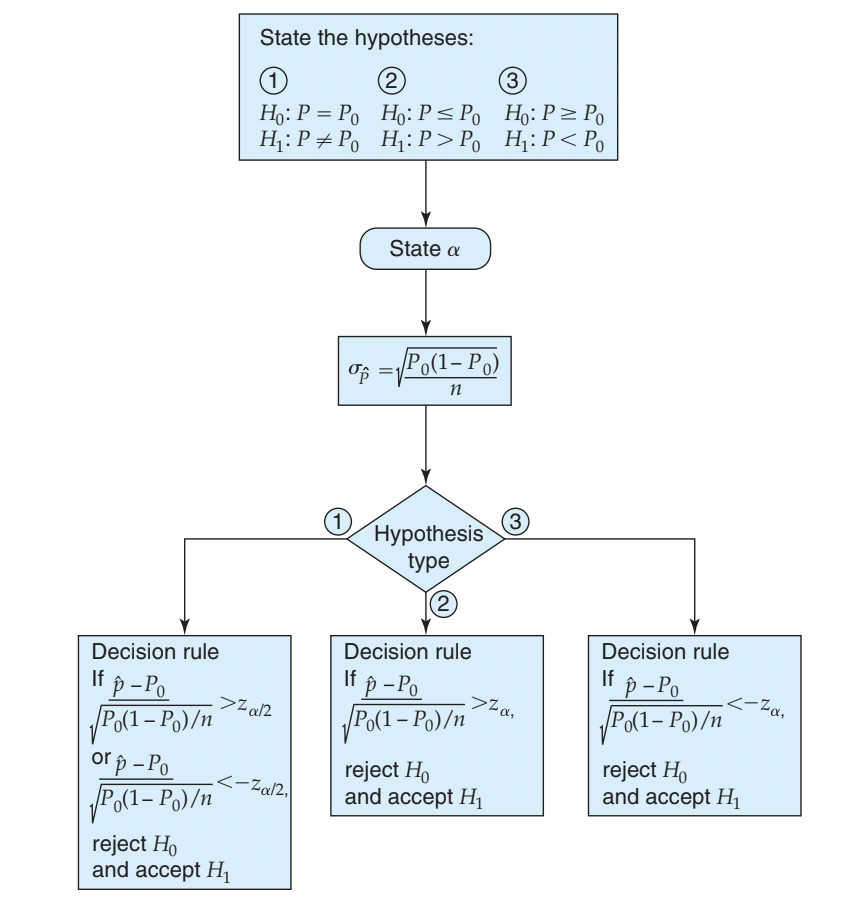
\includegraphics[scale=0.4]{slides6/img/testprop.png}
    \end{center}
\end{frame}

%% Devore 9.11
%\begin{frame}{\color{rosee}Test asint\'otico para una proporci\'on}\small
%  \begin{exampleblock}{Ejemplo (obesidad)}
%    Estudios recientes sugieren que la obesidad es un problema creciente
%    en Estados Unidos en todos los grupos de edades. En una muestra de
%    4115 adultos se reportaron 1276 individuos obesos (un \'indice de masa
%    corporal que excede cierto umbral). Una encuesta de 1998 basada en la
%    opini\'on personal revel\'o que el $20\%$ se consideraba obeso.
%
%    \bigskip ¿Sugieren los datos recientes que la proporci\'on verdadera de
%    adultos obesos 1.5 veces mayor que la reportada en la encuesta de 1998?
%
%    \bigskip Hagamos un test de hip\'otesis de nivel de significaci\'on
%    $\alpha = 0.1$.
%  \end{exampleblock}
%\end{frame}
%
%\begin{frame}{\color{rosee}Test de hip\'otesis para una proporci\'on}\small
%  \begin{exampleblock}{Ejemplo (obsesidad)}
%    Queremos testear
%    \begin{description}
%    \item[$H_0$:] $p = 0.3$
%    \item[$H_1$:] $p > 0.3$
%    \end{description}
%    El estad\'istico del test es
%    \[ Z = \dfrac{\widehat{p} - 0.3}{\sqrt{0.3 \cdot 0.7 /n}}\]
%    Rechazamos $H_0$ si $z\geq z_{0.1} = 1.28$.  La proporci\'on
%    muestral es $1276/4115 = 0.310$, el valor observado del
%    estad\'istico es
%    \[ z_{obs} = (0.31- 0.3) / \sqrt{0.3 \cdot 0.7 /n } = 1.40\] Luego,
%    a nivel $\alpha = 0.1$ hay evidencia suficiente para rechazar la
%    hip\'otesis nula. Es decir que m\'as del $30\%$ de los adultos
%    estadounidenses son obesos.
%  \end{exampleblock}
%\end{frame}

% \begin{frame}{\color{rosee}Test de hip\'otesis para una proporci\'on}\small
%   \begin{exampleblock}{Ejemplo (delivery)}
%     Un servicio de delivery publicita que al menos el $90\%$ de todos
%     los paquetes ordenados antes del mediod\'ia son entregados en el
%     d\'ia. Sea $p$ la proporci\'on poblacional de los paquetes que
%     verifican la publicidad.

%     \medskip
%     Queremos testear
%     \begin{description}
%     \item[$H_0$:] $p = 0.9$
%     \item[$H_1$:] $p < 0.9$
%     \end{description}
%     Si solo el $80\%$ de los paquetes verificaran la publicidad, ¿cu\'an
%     probable es que un test de nivel aproximado $\alpha = 0.1$ basado en
%     una muestra de tama\~no $n=225$ detecte el desv\'io respecto de
%     $H_0$? ¿Qu\'e tama\~no muestral debemos tomar para asegurar que
%     $\beta(0.8)=0.01$?
%   \end{exampleblock}
% \end{frame}

% \begin{frame}{\color{rosee}Test de hip\'otesis para una proporci\'on}\small
%   \begin{exampleblock}{Ejemplo (delivery)}
%     \[\beta(0.8)=1-\Phi\left[\dfrac{0.9-0.8-2.33\sqrt{0.9 0.1
%             /255}}{\sqrt{0.8 0.2 / 225}}\right] = 1-\Phi(2) = 0.228\]
%     Luego, la probabilidad de que $H_0$ sea rechazada usando el test
%     cuando $p=0.8$ es $0.9972$, casi $98\%$ de las muestras llevar\'as
%     al rechazo de $H_0$.
%     \[n = \left[ \dfrac{2.33\sqrt{0.9 0.1} + 2.33 \sqrt{0.8
%             0.2}}{0.8-0.9}\right]^2 \approx 266\]
%   \end{exampleblock}
% \end{frame}

%\subsection{Test de Wald}

\begin{frame}{\color{rosee}Test de Wald}\small

 Podemos construir \textbf{tests
    asint\'oticos} para cualquier par\'ametro $\theta$ usando estimadores \textbf{asintóticamente normales} de $\theta$. Dada una muestra aleatoria
    \[X_1, \dots, X_n \sim f(x;\theta) \text{ con } f \in \mathcal{F} = \{f(x;\theta): \theta \in \Theta \subset
      \mathbb{R}\}\] Queremos realizar el siguiente test
    \[H_0:\theta = \theta_0 \quad\text{vs}\quad H_1: \theta \neq
      \theta_0 \]%\quad (\theta>\theta_{0}, \quad \theta<\theta_{0})\]
 %   Queremos testear
  %  \[H_0: \theta = \theta_0 \text{ vs } H_1: \theta \neq \theta_0\]
    
    Si $\widehat{\theta}_n$ es asint\'oticamente normal y tenemos una
    estimaci\'on consistente de la varianza asint\'otica
    $V(\theta)$. Tomemos, por ejemplo, $V(\widehat{\theta_n})$ el estimador consistente \textit{plug-in} de $V(\theta)$. Consideramos el siguiente estadístico:
    \[W= \dfrac{\sqrt{n}(\widehat{\theta}_n-\theta)}{\sqrt{{\color{dodgerblue}V(\widehat{\theta}_n)}}}\xrightarrow{d}
      N(0,1)\] Dado $\alpha >0$ el test de Wald rechaza
    $H_0$ cuando $\left|\dfrac{\sqrt{n}(\widehat{\theta}_n-\theta_0)}{\sqrt{{\color{dodgerblue}V(\widehat{\theta}_n)}}}\right| > z_{1-\frac{\alpha}{2}}$. 
  
\end{frame}
  
  
\begin{frame}{\color{rosee}Test de Wald}\small
  
En general, 
rechazamos $H_0$ si $W=\dfrac{\sqrt{n}(\widehat{\theta}_n-\theta_0)}{\sqrt{{\color{dodgerblue}V(\widehat{\theta}_n)}}}$ ($W$ bajo $H_0$) cumple que
    \begin{table}
      \begin{tabular}{r|l}
        Hip\'otesis nula & Regi\'on de rechazo \\
        \hline
        $H_0: \theta \leq  \theta_0$ & $W \geq z_{1-\alpha}$ \\
        $H_0: \theta \geq \theta_0$ & $W \leq - z_{1-\alpha}$ \\
        $H_0: \theta =\theta_0$ & $W \geq z_{1-\frac{\alpha}{2}}$ o $W \leq -z_{1-\frac{\alpha}{2}}$\\
      \end{tabular}
    \end{table}  

  
  
 
También se podr\'ia \textbf{(solamente en los casos donde $H_0$ es simple)} considerar el test basado en el estadístico que bajo $H_0$ es
\[\widehat{W}= \dfrac{\sqrt{n}(\widehat{\theta}-\theta_0)}{\sqrt{{\color{dodgerblue}V(\theta_0)}}},\]
  es decir, que no estima la varianza asintótica, sino que usa el valor de la misma bajo la nula. 
  
  
\end{frame}
  
\begin{frame}{\color{rosee}Test de Wald}\small
  \begin{theorem}
    Asint\'oticamente, el test de Wald para $H_0:\theta=\theta_0$ vs $H_1:\theta\neq \theta_0$ tiene nivel asintótico $\alpha$, esto es,
    \[ P_{H_0}(|W|\geq z_{1-\frac{\alpha}{2}}) \xrightarrow{n\to+\infty} \alpha.\]
   % \textbf{Un resultado análogo vale para las otras alternativas.}
  \end{theorem}
  \begin{proof}
    Bajo $H_0$ sabemos que
    \[W=\dfrac{\sqrt{n}\left(\widehat{\theta}_n-\theta_0\right)}{\sqrt{{V(\widehat{\theta}_n)}}} \xrightarrow{d} N(0,1)\]
    Luego, si llamamos $Z\sim N(0,1)$ tenemos que
    \[P_{H_0}(|W| \geq z_{1-\frac{\alpha}{2}}) =
      P_{H_0}\left(\frac{\sqrt{n}|\widehat{\theta}_n-\theta_0|}{\sqrt{{V(\widehat{\theta}_n)}}}\geq z_{1-\frac{\alpha}{2}}
      \right ) \xrightarrow{n\to+\infty} P(|Z| \geq z_{1-\frac{\alpha}{2}}) = \alpha\]
  \end{proof}
\end{frame}

\begin{frame}{\color{rosee}Test de Wald}\small
  
    La \textbf{potencia del test de Wald }para un valor $\theta$ si $H_0:\theta=\theta_0$ vs $H_1:\theta\neq \theta_0$ que tiene nivel $\alpha$, es aproximadamente si $n\gg 0$,
    $$\pi(\theta)=
1- \Phi\left(\frac{\sqrt{n}(\theta_0 -\theta)}{V(\theta)} + z_{1-\frac{\alpha}{2}} \right) +
      \Phi\left(\frac{\sqrt{n}(\theta_0-\theta)}{V(\theta)}- z_{1-\frac{\alpha}{2}} \right)
    $$

 \textbf{ Test de Wald para} $\theta$ \textbf{usando} $\widehat{\theta}_{MV}$

    \begin{description}
    \item[$H_0$:] $\theta = \theta_0$.
    \item[$H_1$:] $\theta \neq \theta_0$.
    \end{description}
Bajo condiciones de regularidad de $\widehat{\theta}_{MV}$, invarianza y Slutsky:
    \[\sqrt{n \cdot \text{I}_1(\widehat{\theta}_{MV})}\, (\widehat{\theta}_{MV}-\theta_0) \xrightarrow{d}
      N(0,1)\] Dado $\alpha >0$ el test de Wald rechaza
    $H_0$ cuando $|W| > z_{1-\frac{\alpha}{2}}$ donde
    \[W= \sqrt{n \cdot \text{I}_1(\widehat{\theta}_{MV})}\, (\widehat{\theta}_{MV}-\theta_0)\]

 \textbf{Como los estimadores de MV son asintóticamente eficientes, los tests de Wald basados en los estimadores de MV serán los tests con mayor potencia asintótica.}
%\begin{itemize}
 %   \item También vale (bajo $H_0$) que:
  %      \[\sqrt{n \cdot \text{I}_1(\theta_0)}\, (\widehat{\theta}-\theta_0) \xrightarrow{d}
   %   N(0,1)\]
    %  \item Puedes usar también como estadístico de contraste: 
     %     \[W= \sqrt{n \cdot \text{I}_1(\theta_0)}\, (\widehat{\theta}-\theta_0)\]
%\end{itemize}  
\end{frame}


\begin{frame}{\color{rosee}Ejemplo con ejercicio 13 del TP5: Test de Wald}\small
  
Se tiene $X_i\stackrel{iid}{\sim}Exp\left(\frac{1}{\theta}\right)$, $\widehat{\theta}_{MV}=\overline{X}_n$, $\beta(\theta)=P(X>3)=e^{-\frac{3}{\theta}}$ e $I_1^{-1}(\theta)=\theta^2$. 

Dé la región de rechazo del test de Wald de nivel 5\% para la hipótesis $$H_0: \beta(\theta)=0.5 \quad vs \quad H_1: \beta(\theta)\neq 0.5$$ 
 ¿Qué decisión se toma para los datos que se observan $\overline{x}_{100}=1.4$? 

 \color{gray}
\[\mathcal{R}=\left\{\left|\beta(\widehat{\theta}_{MV})-0.5\right|>z_{1-\frac{\alpha}{2}}\cdot \sqrt{3}\widehat{\theta}_{MV}^{-1}\cdot e^{-3/\widehat{\theta}_{MV}}\right\}\]

Para los datos, $\beta(\widehat{\theta}_{MV,obs})=e^{-\frac{3}{1.4}}\approx 0.1173191$, $z_{0.975}=1.96$, entonces:
\begin{itemize}
    \item $\left|\beta(\widehat{\theta}_{MV})-0.5\right|\approx 0.38268$
    \item $z_{0.975}\cdot \sqrt{3}\widehat{\theta}_{MV}^{-1}\cdot e^{-3/\widehat{\theta}_{MV}}\approx 0.2844838589$
\end{itemize}

Entonces se rechaza $H_0$ del test bilateral con un nivel $\alpha=0.05$.
\color{black}

  
  
\end{frame}


\begin{frame}{\color{rosee}Ejemplo con ejercicio 13 del TP5: Test de Wald}\small


 Repita el análisis para la hipótesis $H_0: \beta(\theta)=1/2$ vs $H_1: \beta(\theta)> 1/2$.
 
 \color{gray}
\[\mathcal{R}=\left\{\beta(\widehat{\theta}_{MV})-0.5>z_{1-\alpha}\cdot \sqrt{3}\widehat{\theta}_{MV}^{-1}\cdot e^{-3/\widehat{\theta}_{MV}}\right\}\]

Para los datos, $\beta(\widehat{\theta}_{MV,obs})=e^{-\frac{3}{1.4}}\approx 0.1173191$, $z_{0.95}=1.645$, entonces:
\begin{itemize}
    \item $\beta(\widehat{\theta}_{MV})-0.5\approx -0.38268$
    \item $z_{0.95}\cdot \sqrt{3}\widehat{\theta}_{MV}^{-1}\cdot e^{-3/\widehat{\theta}_{MV}}\approx 0.238763$
\end{itemize}
Entonces no se rechaza $H_0$ del test a cola derecha con un nivel $\alpha=0.05$.

\color{black}

  \vspace{10pt}
  
  ¿Se podría haber realizado este test de hipótesis sin suponer el modelo exponencial para los datos?
  
\color{gray}

\vspace{10pt}

  Sí, consideremos el test bilateral. Hay que definir $W_i=I_{(3,+\infty)}(X_i)\stackrel{iid}{\sim}Be(p)$ donde $p=P(X_i>3)=\beta(\theta)$, colectar una muestra de datos $w_i$ (en este caso no lo tenemos) y conducir un test para $p$.
  
  
\end{frame}

%\begin{frame}{\color{rosee}Relación entre tests bilaterales e IC}\small
    
   %   El test de Wald de nivel $\alpha$ rechaza $H_0: \theta = \theta_0$
   %   en favor de $H_1: \theta \neq \theta_0$ si y s\'olo si
    %  $\theta_0 \notin IC_{\theta}^{(1-\alpha)100\%}$ donde
     % \[ IC_{\theta}^{(1-\alpha)100\%}= \left[\widehat{\theta}- z_{1-\frac{\alpha}{2}}V(\widehat{\theta}) ,
      %    \widehat{\theta}+ z_{1-\frac{\alpha}{2}}V (\widehat{\theta}) \right] \]
    
      %Realizar un test a dos colas es equivalente a ver si el valor del parámetro en la  hip\'otesis nula pertenece al intervalo de confianza.

 % Dado un test de nivel $\alpha$ para las hip\'otesis
 %\[H_0: \theta = \theta_0 \quad\text{vs}\quad H_1: \theta \neq
  % \theta_0\] y una muestra $\munderbar{X}$, llamemos $C(\munderbar{X})$ a aquellos valores
% poblacionales $\theta_0$ para lo cuales el test evaluado en la muestra
 %$\mathbf{X}$ rechazar\'ia $H_0$. Es decir,
 %\[C(\munderbar{X}) = \{ \widetilde{\theta}: \mbox{no rechazo } H_0: \theta =
 %  \widetilde{\theta} \mbox{ para la muestra } \mathbf{X}\}\] %(es un conjunto aleatorio porque depende de la muestra).
 %Vemos que
 %\[P_{\theta_0} (\theta_0 \in C(\munderbar{X})) = P_{\theta_0} (\mbox{no rechazo } H_0)= 1-P_{\theta_0}(\mbox{rechazo $H_0$}) = 1-\alpha\] Entonces %$C(\munderbar{X})$
% es una regi\'on de confianza de nivel $1-\alpha$ obtenida a partir de
% invertir el test.
%\end{frame}

%\begin{frame}{\color{rosee}Relaci\'on con intervalos de confianza}\small
%  \begin{block}{Test - intervalos}
%    \begin{itemize}
%    \item Cuando el valor del par\'ametro dado en $H_0$ cae fuera de un
%      intervalo de confianza del $100(1-\alpha)\%$, deber\'iamos
%      rechazar $H_0$ en un test de hip\'otesis con nivel de
%      significaci\'on $\alpha$.
%    \item Cuando el valor del par\'ametro especificado por $H_0$ cae
%      dentro del intervalo de confianza del $100(1-\alpha)\%$, no
%      tendr\'iamos evidencia suficiente para rechazar $H_0$ en un test
%      de hip\'otesis de nivel $\alpha$.
%    \end{itemize}
%  \end{block}
%\end{frame}




% \begin{frame}{\color{rosee}\small
%   Bajo condiciones de regularidad, para $n\rightarrow \infty$,
%   $$\sqrt{n}(\widehat\theta_{MV} - \theta_0) \xrightarrow{\mathcal{L}}
%   \mathcal{N}(0,I^{-1}(\theta_0)$$
%   equivalentemente
%   $$ \frac{\sqrt{n}(\widehat\theta_{MV}-\theta_0)}{\sqrt{I^{-1}(\theta_0)}}
%   \xrightarrow{\mathcal{L}} N(0,1)$$
%   Entonces, elevamos al cuadrado y obtenemos
%   $$ W_1 = n(\widehat\theta_{ML} - \theta_0)^2 I(\theta_0) \xrightarrow{\mathcal{L}}
%   \chi_1^2 $$
% \end{frame}
%
% \begin{frame}{\color{rosee}Test de Wald}\small
%   Adem\'as, si $I$ es continua como funci\'on de $\theta$,
%   $$I(\widehat\theta_{MV})/I(\theta_0) \xrightarrow{P_{\theta_0}} 1$$
%   pues
%   $$\widehat\theta_{MV} \xrightarrow{P_{\theta_0}} \theta_0$$
%   Por el teorema  de Slutsky
%   $$ W_2 = I(\widehat\theta_{MV})n(\widehat\theta_{MV}-\theta_0)^2 =
%   \left(\frac{I(\widehat\theta_{MV})}{I(\theta_0)} \right) W_1
%   \xrightarrow{\mathcal{L}} \chi^2_1$$
% \end{frame}

% \begin{frame}{\color{rosee}Test de Wald}\small
%   Por otro lado, por LGN
%   $$ i(\theta) = -\frac{1}{n}\sum_{i=1}^n \frac{d^2}{d\theta^2} \log
%   f(x;\theta) \xrightarrow{P_{\theta_0}} I(\theta) =
%   -E_{\theta}\left(\frac{d^2}{d\theta^2} \log
%     f(x;\theta) \right)$$
%   Entonces, 
%   $$i(\theta)/I(\theta) \xrightarrow{P_{\theta_0}} 1$$
%   y, por el teorema de Slutsky,
%   $$ W_3 = i(\theta_0)n(\widehat\theta_{MV} - \theta_0)^2 =
%   \left(\frac{i(\theta_0)}{I(\theta_0)}\right) W_1
%   \xrightarrow{\mathcal{L}} \chi^2_1$$
% \end{frame}

% \begin{frame}{\color{rosee}Test de Wald}\small
%   A su vez, 
%   $$i(\widehat\theta_{MV}) = -\frac{1}{n} \sum_{i=1}^n \frac{d^2}{d\theta^2}
%   \log f(x;\theta)|_{\theta = \widehat\theta_{MV}} = i(\theta_0) -
%   \underbrace{\frac{1}{n}\log'''(\widetilde\theta)
%   (\widehat\theta_{MV}-\theta)}_{\xrightarrow{P_{\theta_0}}
%   0}$$
%   con $\widetilde\theta$ entre $\widehat\theta_{MV}$ y $\theta$.  Entonces
%   $i(\widehat\theta_{MV})/I(\theta_0) \xrightarrow{P_{\theta_0}} 1$ y
%   por
%   Slutsky
%   $$ W_4= i(\widehat\theta_{MV}) n(\widehat\theta_{MV}-\theta_0)^2 =
%   \frac{i(\widehat\theta_{MV})}{I(\theta_0)} W_1 \xrightarrow{\mathcal{L}}
%   \chi^2_1$$
%   Entonces, un test de Wald es un test cuya regi\'on de rechazo de $H_0$
%   es de la forma $W_j \geq \chi^2_1$ de manera que
%   $$P_{\theta_0}(W_j \geq \chi_{1,\alpha})^2) \rightarrow \alpha$$
%   para $j=1,2,3,4$ cuando $n\rightarrow \infty$.
% \end{frame}

%
%
%\subsection{Test de cociente de verosimilitud}
%
%\begin{frame}{\color{rosee}Distribuci\'on $\chi^2$}\small
%  \begin{definition}[chi cuadrado con $k$ grados de libertad]
%    Si $Z_1, Z_2, \dots, Z_k$ son variables aleatorias independientes tales que
%    $Z_i \sim N(0,1)$ entonces decimos que
%    \[\sum_{i=1}^k Z_i^2 \sim \chi^2_k\]
%  \end{definition}
%  \begin{block}{}
%    \begin{itemize}
%    \item Es una variable positiva.
%    \item Dado un vector en $\mathbb{R}^n$ cuyas coordenadas se generan
%      de manera normal est\'andar y son independientes, su norma al cuadrado se distribuye
%      como $\chi^2_n$.
%    \item Si $X \sim \chi^2_k$, $E(X)=k$ y $Var(X)=2k$.
% 
%    \end{itemize}
%  \end{block}
%\end{frame}

%\begin{frame}{\color{rosee}Distribuci\'on $\chi^2$}\small
%  \begin{figure}
%    \centering
%    \includegraphics[height=.9\textheight]{img/chisq.pdf}
%  \end{figure}
%\end{frame}
%
%\begin{frame}{\color{rosee}Test del cociente de verosimilitud}\small
%  \begin{block}{Test del cociente de verosimilitud}
%    Si queremos testear
%    \begin{description}
%    \item[$H_0$:] $\theta = \theta_0$.
%    \item[$H_1$:] $\theta \neq \theta_0$.
%    \end{description}
%    El estad\'istico del test es
%    \[\lambda(X) =
%      % 2\log \left(\dfrac{\max_{\theta}\mathcal{L}(\theta)}{\sup_{\theta \in
%      %       \Theta_0}\mathcal{L}(\theta)}\right)
%      2\log\left(\frac{\mathcal{L}(\widehat{\theta}_{MV})}{
%          \mathcal{L}(\theta_0)}\right)\]
%    donde $\widehat{\theta}_{MV}$ es el EMV de $\theta$.
%    % y $\widehat{\theta_0}$ es el EMV
%    % cuando $\theta$ se restringe a $\theta_0$.
%
%    \bigskip Es equivalente a mirar la diferencia entre
%    log-verosimilitudes
%    \[2\left[
%        \log\left(\mathcal{L}\left(\widehat{\theta}_{MV}\right)\right)-
%        \log\left(\mathcal{L}\left(\theta_0\right)\right)\right ]\] El
%    test rechaza $H_0$ cuando $\lambda(X)$ es grande.
%  \end{block}
%\end{frame}
%  
%\begin{frame}{\color{rosee}Test del cociente de verosimilitud}\small
%  \begin{theorem}
%    Bajo condiciones de regularidad, para $n \rightarrow \infty$,
%    \[ P_{\theta_0} \left(\lambda(X) \geq
%        \chi_{1,1-\alpha}^2\right)\rightarrow \alpha \] es decir que el
%    test para $H_0: \theta=\theta_0$, tiene nivel asint\'otico $\alpha$.
%  \end{theorem}
%\end{frame}
%
%\begin{frame}{\color{rosee}Test del cociente de verosimilitud}\small
%  \begin{block}{Demostraci\'on}
%    Un desarrollo de Taylor de segundo orden alrededor de
%    $\widehat{\theta}_{MV}$ resulta
%    \begin{align*}
%      2\log\mathcal{L}(\theta_0) = 2\log\mathcal{L}\left(\widehat\theta_{MV}\right)
%      &+ \underbrace{2\left(\log\mathcal{L}(\theta)\right)'\Big|_{\theta=\widehat\theta_{MV}}}_{=0}
%        \left(\theta_0-\widehat\theta_{MV}\right)\\
%      &+ \frac{1}{2} 2\left(\log\mathcal{L}(\theta)\right)''\Big|_{\theta = \widetilde\theta} \left(\theta_0-\widehat\theta_{MV}\right)^2
%    \end{align*}
%    con $\widetilde\theta$ entre $\theta_0$ y $\widehat\theta_{MV}$.
%    \scriptsize
%    \begin{align*}
%      \lambda(X)
%      &= 2\log\mathcal{L}\left(\widehat{\theta}_{MV}\right) - 2\log\mathcal{L}(\theta_0) =
%        - \frac{1}{n} 
%        \left(2\log \mathcal{L}(\theta)\right)''\Big|_{\theta = \widetilde{\theta}}\left[\sqrt{n}
%        \left(\theta_0-\widehat{\theta}_{MV} \right)\right]^2\\
%      &= \underbrace{\left(\frac{\sqrt{n}
%        \left(\theta_0-\widehat{\theta}_{MV}\right)}{\sqrt{I^{-1}(\theta_0)}}\right)^2}_{(A)}
%        + \underbrace{\left ( -I(\theta) - \frac{1}{n} \left(\log\mathcal{L}\left(\widetilde{\theta}\right)\right)''\Big|_{\theta=\widetilde{\theta}}
%        \right)\left(\sqrt{n}(\theta_0 - \widehat{\theta}_{MV})\right)^2}_{(B)}
%    \end{align*}
%    \small
%    El t\'ermino $(A)$, por el TCL, tiende en distribuci\'on a una
%    $\chi^2_1$.
%  \end{block}
%\end{frame}
%
%\begin{frame}{\color{rosee}Test del cociente de verosimilitud}\small
%  \begin{block}{Demostraci\'on}
%    Para el t\'ermino $(B)$ hagamos un desarrollo de primer orden
%    alrededor de $\theta_0$:
%    \[\frac{1}{n}\left(\log\mathcal{L}(\theta)\right)''\Big|_{\theta=\widetilde\theta} =
%        \underbrace{\frac{1}{n}\left(\log\mathcal{L}(\theta)\right)''\Big|_{\theta=\theta_0}}_{\rightarrow -I(\theta_0)} +
%    \underbrace{\frac{1}{n}\left(\log\mathcal{L}(\theta)\right)'''
%      \Big|_{\theta=\widetilde{\widetilde\theta}}(\widetilde\theta -
%      \theta_0)}_{\xrightarrow{P_{\theta_0}} 0}\] con
%    $\widetilde{\widetilde\theta}$ entre $\widetilde\theta$ y $\theta_0$. Adem\'as,
%    \[ \left[\sqrt{n}\left(\theta_0 - \widehat\theta_{MV}\right)\right]^2
%    \cw \mathcal{N}(0,I^{-1}(\theta_0))\] Por el teorema de
%    Slutsky, $(B)\cw 0$ y entonces
%    $$\lambda(X) \cw \chi^2_1$$
%  \end{block}
%\end{frame}
%
%% \subsection{Test de score (o multiplicador de Lagrange)}
%
%% \begin{frame}{\color{rosee}Test de score (o multiplicador de Lagrange)}\small
%%   Sea $s(X;\theta_0)$ el \textit{score} basado en toda la muestra
%%   evaluado en $\theta_0$ y sea $I(\theta_0)$ la informaci\'on de una
%%   unidad de observaci\'on. Entonces
%%   $$ \frac{s(X;\theta_0)}{\sqrt{nI(\theta_0)}} \xrightarrow{\mathcal{L}}
%%   N(0,1)$$
%%   Elevando al cuadrado
%%   $$
%%   \underbrace{\left(\frac{s(X;\theta_0)}{\sqrt{nI(\theta_0)}}\right)^2}_{T_1(X)}
%%   \xrightarrow{\mathcal{L}} \chi^2_1$$
%%   El test rechaza si $T_1(X) > \chi^2_{1,\alpha}$. Una alternativa es 
%%   $$ T_2(X) = \frac{1}{n} \frac{s^2(X;\theta_0)}{i(\theta_0)}$$
%%   con $i(\theta_0)= -\frac{1}{n} \sum_{i=1}^n \frac{d^2}{d\theta^2} \log
%%   f(X_i;\theta)$.
%% \end{frame}
%
%\begin{frame}{\color{rosee}Test de cociente de verosimilitud}\small
%  En general, podemos preguntarnos si un par\'ametro multidimensional
%  $\theta \in \Theta \subset \mathbb{R}^n$ pertenece a un subconjunto
%  m\'as chico $\Theta_0 \subset \Theta$:
%  \begin{description}
%  \item[$H_0$:] $\theta \in \Theta_0$
%  \item[$H_1$:] $\theta \notin \Theta_0$
%  \end{description}
%  En este caso, el estad\'istico se generaliza como el cociente de los estimadores en cada caso:
%  \[\lambda(X) = 2\log\left(\frac{\sup_{\theta \in \Theta}
%        \mathcal{L}(\theta)}{\sup_{\theta \in \Theta_0}
%        \mathcal{L}(\theta)}\right) = 2\log
%    \left(\dfrac{\mathcal{L}(\widehat{\theta}_{MV})}{\mathcal{L}(\widehat{\theta}_0)}\right)\]
%  donde $\widehat{\theta}_{MV}$ es el EMV de $\theta$ y
%  $\widehat{\theta_0}$ es el EMV cuando $\theta$ se restringe a
%  $\theta_0$.
%\end{frame}
%
%\begin{frame}{\color{rosee}Test de cociente de verosimilitud}\small
%    \begin{exampleblock}{Ejemplo} % Devore 9.24
%      Dada una muestra aleatoria $X_1,\dots,X_n \sim
%      \mathcal{N}(\mu,\sigma^2)$ con $\mu$ y $\sigma$ desconocidos
%      ($\theta=(\mu,\sigma)$). Queremos testear
%      $$H_0: \mu=\mu_0 \quad\text{vs}\quad H_1: \mu \neq \mu_0$$
%      Para usar el test de cociente de verosimilitud necesitamos
%      \begin{itemize}
%      \item el EMV en todo el espacio de par\'ametros
%        \[(\widehat\mu_{MV}, \widehat\sigma^2_{MV}) = (\overline X,
%          \frac{1}{n} \sum_{i=1}^n (X_i-\overline X)^2)\]
%      \item y el EMV bajo la hip\'otesis nula
%        \[(\widehat\mu_{R}, \widehat\sigma^2_{R}) = (\mu_0, \frac{1}{n}
%        \sum_{i=1}^n (X_i- \mu_0)^2)\]
%      \end{itemize}
%    \end{exampleblock}
%  \end{frame}
%
%  \begin{frame}{\color{rosee}Test de cociente de verosimilitud}\small
%    \begin{exampleblock}{} \scriptsize
%      El estad\'istico del test resulta:
%      \begin{align*}
%        \lambda(X) &= \left(\frac{\widehat\sigma_{MV}^{-2}}{\widehat\sigma_R^{-2}}
%                     \right)^{n/2} \exp
%                     \left[-\frac{1}{2\widehat\sigma^2_{MV}} \sum_{i=1}^n
%                     (X_i-\widehat\mu_{MV})^2 + \frac{1}{2\widehat\sigma^2_R}
%                     \sum_{i=1}^n(X_i -\mu_0)^2\right]\\
%                   &= \frac{\widehat\sigma_R^2}{\widehat\sigma_{MV}^2}^{n/2} =
%                     \left(\frac{\sum_{i=1}^n (X_i-\mu_0)^2}{\sum_{i=1}^n
%                     (X_i- \overline X)^2} \right)^{n/2} = \left(1+
%                     \frac{n(\overline X - \mu_0)^2}{\sum_{i=1}^n
%                     (X_i - \overline X)^2}\right)^{n/2}\\
%                   &= \left(1+
%                     \frac{1}{n-1}\left[\underbrace{\frac{\sqrt{n}(\overline
%                     X-\mu_0)}{S}}_{=T}\right]^2\right)^{n/2} = \left(1+
%                     \frac{1}{n-1}T^2 \right )^{n/2} = g \left(T^2\right)
%      \end{align*}
%      con $g(u) = \left(1+ \frac{1}{n-1} u \right)^{n/2}$ creciente. Luego
%      \[g \left(T^2 \right) \geq k_1 \Leftrightarrow T^2 \geq k_2 \Leftrightarrow |T| >
%      k_3\]
%      En este caso, sabemos que $T \sim t_{n-1}$ y no es necesario
%      recurrir a la distribuci\'on asint\'otica. Es decir, el test $T$ es el
%      test del cociente de m\'axima verosimilitud para el caso normal.
%    \end{exampleblock}
%  \end{frame}
%
%  \begin{frame}{\color{rosee}Test de cociente de verosimilitud} \small
%    \begin{exampleblock}{Ejemplo (cociente de verosimilitud)} % Devore 9.25
%      Sea $X_1, \dots, X_n$ una muestra aleatoria de $n$ errores de
%      medici\'on de cierta caracter\'istica f\'isica tal que
%      \[f(x) = \frac{1}{2} e^{-|x-\theta|}\] 
%      Queremos testear $H_0: \theta=0$ contra
%      $H_1: \theta \neq 0$. La verosimilitud es
%      \[L(\theta) = \frac{1}{2^n} e^{- \sum_{i=1}^n \left |x_i-\theta \right |}\]
%      Ya vimos que $\widehat{\theta}_{MV} = m_n = mediana(X_1,\dots,X_n)$.
%    \end{exampleblock}
%  \end{frame}
%  
%  \begin{frame}{\color{rosee}Test de cociente de verosimilitud} \small
%    \begin{exampleblock}{Ejemplo (cociente de verosimilitud)} % Devore 9.25
%      El estad\'istico del test es, bajo $H_0: \theta=0$,
%      \begin{align*}
%        2\log\left [\frac{L(\widehat{\theta}_{MV})}{L(\theta_0)}\right ]
%        &= 2\log \left(\frac{e^{-\sum_{i=1}^n \left|x_i-m_n \right|}}{e^{-\sum_{i=1}^n \left|x_i\right |}}\right)\\
%        &= 2 \left(\sum_{i=1}^n |x_i| - \sum_{i=1}^n |x_i - m_n | \right)
%      \end{align*}
%      Si tuvi\'eramos $n=30$,
%      $\sum_{i=1}^n |x_i| = 38.6$ y $\sum_{i=1}^n |x_i-m_n| = 37.3$
%      entonces
%      \[2\log(L) = 2.6 < \chi^2_{1,1-0.05} = 3.84\] no hay evidencia para
%      rechazar $H_0$ a nivel $5\%$. no podemos descartar que las mediciones
%      tuvieran sesgo.
%      \end{exampleblock}
%    \end{frame}
%    
%  % \begin{frame}{\color{rosee}Algunos resultados}\small
%  %   \begin{block}{Equivalencia}
%  %     Puede probarse que bajo $H_0$ la diferencia entre cualquier par de
%  %     estadísticos de los tres tests vistos tiende a cero en probabilidad
%  %     cuando $n\rightarrow \infty$. Entonces con una probabilidad alta,
%  %     las regiones de rechazo de todos estos tests son muy parecidas
%  %     (cuando $n$ es grande y $H_0$ es verdadera).
%  %   \end{block}
%  %   \begin{block}{Potencia}
%  %     Puede probarse que bajo ciertas condiciones de regularidad
%  %     $$P_{\theta_1}(W_1 > k) \rightarrow 1 (n\rightarrow \infty)$$
%  %   \end{block}
%  % \end{frame}
%
%  % \begin{frame}{\color{rosee}Invariancia ante reparametrizaciones}\small
%  %   \begin{exampleblock}{Wald no es invariante por reparametrizaciones del modelo.}
%  %     Dada una muestra aleatoria $X_1,\dots,X_n \sim Bin(1,\theta)$
%  %     testeamos
%  %     \[H_0 : \theta = 1/3 \quad\text{vs}\quad H_1:\theta \neq 1/3\] El
%  %     estadístico del test de Wald es
%  %     $$W_1 = \left[\frac{\sqrt{n}(\overline X -
%  %         1/3)}{\sqrt{I(1/3)^{-1}}}\right]^n$$
%  %     con 
%  %     $$ I(1/3)=-E_{\theta=1/3}\left(\frac{d^2}{d\theta^2}\log f|_{\theta
%  %         = 1/3}\right)$$
%  %   \end{exampleblock}
%  % \end{frame}
%
%  \begin{frame}{\color{rosee}Invariancia ante reparametrizaciones}\small
%    % \begin{exampleblock}{}
%    %   Si reparametrizamos el modelo con $\tau = \sqrt[3]{\theta}$ entonces
%    %   las hip\'otesis son
%    %   $$\widetilde H_0 : \tau = \sqrt[3]{1/3} \quad\text{vs}\quad \widetilde
%    %   H_1:\tau \neq \sqrt[3]{1/3}$$
%    %   y el estadístico
%    %   $$\widetilde W_1 = \left[\frac{\sqrt{n}(\sqrt[3]{\overline X} -
%    %       \sqrt[3]{1/3})}{\sqrt{\widetilde I(\sqrt[3]{1/3})^{-1}}}\right]^n$$
%    %   con
%    %   $$\widetilde
%    %   I(\sqrt[3]{1/3})=-E_{\tau=\sqrt[3]{1/3}}\left(\frac{d^2}{d\theta^2}\log
%    %     f|_{\tau = \sqrt[3]{1/3}}\right)$$
%    %   $W_1$ y $\widetilde W_1$ son variables distintas, una es funci\'on lineal
%    %   de $\overline X$ y la otra no. 
%    % \end{exampleblock}
%    \begin{alertblock}{}
%      \begin{itemize}
%      \item El test de Wald no es invariante por reparametrizaciones del
%        modelo.
%      \item La propiedad de invariancia del estimador de MV asegura que el test del
%        cociente de verosimilitud sea invariante por reparametrizaciones
%        del modelo.
%      \end{itemize}
%    \end{alertblock}
%  \end{frame}
%
%
%  % \begin{frame}{\color{rosee}Invariancia ante reparametrizaciones}\small  
%  %   \begin{itemize}
%  %   \item La propiedad de invariancia del EMV asegura que el test del
%  %     cociente de verosimilitud sea invariante por reparametrizaciones del
%  %     modelo.
%  %   \item Veamos que el test de score tambi\'en es invariante. Consideremos una
%  %     reparametrizaci\'on $\theta = g(\tau)$ con $g$ diferenciable
%  %     $$f(x_i;\theta) = f(x_i;g(\tau)) = \widetilde f(x_i;\tau)$$
%  %     Regla de la cadena
%  %     \begin{align*}
%  %       \widetilde s(x_i;\tau) 
%  %       &= \frac{d}{d\tau}\log \widetilde f(x_i;\tau) =
%  %         \frac{d}{d\tau}\log f(x_i;g(\tau)) \\ 
%  %       &= \frac{d}{d\tau}\log f(x_i;\theta)|_{g(\tau)}
%  %         \frac{d}{d\tau}g(\tau)
%  %     \end{align*}
%  %     Entonces 
%  %     $$\widetilde s(x_i;\tau) = s(x_i,\theta) \frac{d}{d\tau}g(\tau)$$
%  %   \end{itemize}
%  % \end{frame}
%
%  % \begin{frame}{\color{rosee}Invariancia ante reparametrizaciones}\small  
%  %   An\'alogamente
%  %   $$\widetilde I (\tau)= E(\widetilde s(x_i;\tau)^2) = E(s(x_i;\theta)^2) \left
%  %     [\frac{d}{d\tau}g(\tau)\right]^2 =
%  %   I(\theta)\left[\frac{d}{d\tau}g(\tau) \right]^2$$
%  %   Si $\theta = g(\tau_0)$, reemplazando
%  %   $$\frac{1}{n} \frac{\sum_{i=1}^n \widetilde s(x_i,\tau_0)}{\widetilde
%  %     I(\tau_0)} = \frac{1}{n} \frac{\sum_{i=1}^n
%  %     s^2(x_i;\theta_0)}{I(\theta_0)}$$
%  %   Entonces el test de score es invariante por reparametrizaciones del modelo.
%  % \end{frame}
%
% 

\end{document}